\documentclass{article}
\usepackage{amsmath}
\usepackage{graphicx}
\usepackage{amsfonts}
\usepackage{amssymb}
\usepackage{bm}
\usepackage[colorlinks=true, linkcolor=black, urlcolor=blue]{hyperref}
\usepackage{fontspec}
\setmainfont{Times New Roman}
\usepackage{microtype}
\emergencystretch=2em
\usepackage{listings}
\usepackage{xcolor}
\usepackage{mathtools}
\usepackage{tcolorbox}
\tcbuselibrary{breakable}
\usepackage{fancyvrb}
\usepackage{placeins}
\usepackage{booktabs}
\usepackage{float}
\usepackage[a4paper, margin=1in]{geometry}
\usepackage{subcaption}
\usepackage{tikz}
\usetikzlibrary{arrows.meta,positioning,fit,backgrounds,calc}
\usepackage{pgfplots}
\pgfplotsset{compat=1.18}
\usepackage{float}
\usepackage[backend=biber, style=ieee, sorting=none]{biblatex}
\addbibresource{references.bib}
% ---------- COLORS ----------
\definecolor{inputblue}{RGB}{66,165,245}
\definecolor{sigmoidpurple}{RGB}{171,71,188}
\definecolor{hidden1}{RGB}{129,199,132}
\definecolor{hidden2}{RGB}{255,193,7}
\definecolor{reluorange}{RGB}{255,167,38}
\definecolor{bncyan}{RGB}{0,188,212}
\definecolor{outputred}{RGB}{244,67,54}
\definecolor{residualgray}{RGB}{96,125,139}
\definecolor{normalpink}{RGB}{192,57,70}
\definecolor{anemicpale}{RGB}{236,207,203}

% ---------- TIKZ STYLES ----------
\tikzset{
	>=Latex,
	neuron/.style={
		circle,
		draw,
		thick,
		minimum size=7mm,
		inner sep=0pt
	},
	layerbox/.style={
		draw,
		rounded corners,
		thick,
		inner sep=4pt,
		fill opacity=0.06
	},
	conn/.style={
		-{Latex[length=2mm,width=1.6mm]},
		line width=0.6pt
	}
}


\lstset{
	language=Matlab,
	basicstyle=\small\ttfamily,
	keywordstyle=\color{blue},
	commentstyle=\color{green!70!black},
	stringstyle=\color{red},
	showstringspaces=false,
	frame=single,
	captionpos=b,
	% --- ADD THESE THREE LINES TO FIX LINE BREAKING ---
	breaklines=true,                 % 1. Enables automatic line breaking
	breakatwhitespace=false,         % 2. Allows breaking lines at non-whitespace
	postbreak=\mbox{\textcolor{red}{$\hookrightarrow$}\space} % 3. Adds an arrow to show a line break
}

\begin{document}
	\begin{titlepage}
		\centering
		\includegraphics[width=0.3\textwidth]{download.png} \\[1.5cm]
		{\huge \textbf{K.N. Toosi University}}\\[2cm]
		{\Large \textbf{Aidin Sahneh}}\\[0.5cm] 
		{\large \textbf{Student ID:} 40120243}\\[0.7cm]
		{\Large \textbf{Amir Hosseinpoor}}\\[0.5cm] 
		{\large \textbf{Student ID:} 40117393}\\[0.7cm]
		{\Large \textbf{Mani Vafapour} (Intro to ML) }\\[0.2cm] 
		{\large \textbf{\\ Student ID:} 40123783}\\[0.7cm]
		{\Large \textbf{Amirhossein Shaqaqi} (Robotics \& Vision) }\\[0.5cm] 
		{\large \textbf{Student ID:}  40119843}\\[0.7cm]
		{\Large \textbf{Course:} Robotics \& Computer Vision / Intro to ML}\\[0.3cm]
		{\large \textbf{Instructors:} Prof. Taghirad \& Dr. Nikoofard \& Dr. Ahmadi }\\[1cm]
		
		
		
		
	\end{titlepage}
	
	\newpage
	\tableofcontents
	\newpage
	
	
	
	
	
	\begin{latin}
		\section{Data Curation and Preprocessing (\texttt{classification/datapreparepipeline/})}
		\label{sec:data-curation}
		
		The data curation and preprocessing pipeline is responsible for transforming raw clinical conjunctival photographs and laboratory blood records into a mathematically clean, leak-free, and balanced dataset ready for deep learning training and evaluation.
		
		\begin{figure}[htbp]
			\centering
			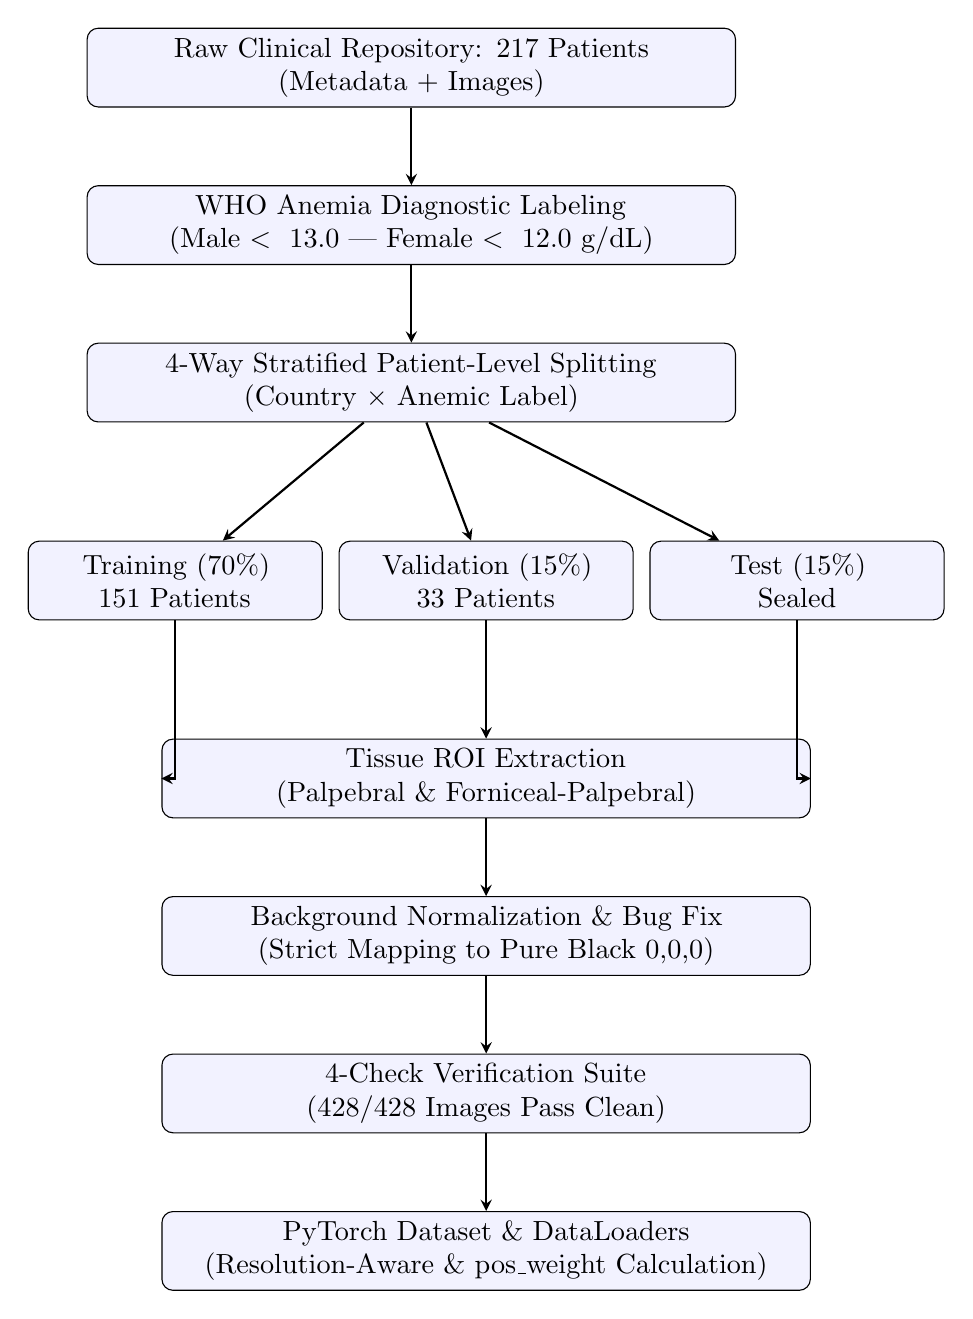
\begin{tikzpicture}[
				node distance=1.5cm,
				box/.style={rectangle, draw, rounded corners, align=center, fill=blue!5, text width=8cm, minimum height=1cm},
				arrow/.style={thick,->,>=stealth}
				]
				\node (A) [box] {Raw Clinical Repository: 217 Patients\\(Metadata + Images)};
				\node (B) [box, below of=A, yshift=-0.5cm] {WHO Anemia Diagnostic Labeling\\(Male $< 13.0$ | Female $< 12.0$ g/dL)};
				\node (C) [box, below of=B, yshift=-0.5cm] {4-Way Stratified Patient-Level Splitting\\(Country $\times$ Anemic Label)};
				
				\node (D) [box, below left=1.5cm and -3cm of C, text width=3.5cm] {Training (70\%)\\151 Patients};
				\node (E) [box, right=0.2cm of D, text width=3.5cm] {Validation (15\%)\\33 Patients};
				\node (F) [box, right=0.2cm of E, text width=3.5cm] {Test (15\%)\\Sealed};
				
				\node (G) [box, below=1.5cm of E] {Tissue ROI Extraction\\(Palpebral \& Forniceal-Palpebral)};
				\node (H) [box, below of=G, yshift=-0.5cm] {Background Normalization \& Bug Fix\\(Strict Mapping to Pure Black 0,0,0)};
				\node (I) [box, below of=H, yshift=-0.5cm] {4-Check Verification Suite\\(428/428 Images Pass Clean)};
				\node (J) [box, below of=I, yshift=-0.5cm] {PyTorch Dataset \& DataLoaders\\(Resolution-Aware \& pos\_weight Calculation)};
				
				\draw [arrow] (A) -- (B);
				\draw [arrow] (B) -- (C);
				\draw [arrow] (C) -- (D);
				\draw [arrow] (C) -- (E);
				\draw [arrow] (C) -- (F);
				\draw [arrow] (D) |- (G);
				\draw [arrow] (E) -- (G);
				\draw [arrow] (F) |- (G);
				\draw [arrow] (G) -- (H);
				\draw [arrow] (H) -- (I);
				\draw [arrow] (I) -- (J);
			\end{tikzpicture}
			\caption{Architecture of the data curation and preprocessing pipeline.}
			\label{fig:data_pipeline}
		\end{figure}
		
		\subsection{Source Data and Clinical Origin}
		This project operates on the \textbf{Eyes-Defy-Anemia} clinical dataset, which includes non-invasive conjunctival photographs and laboratory blood hemoglobin (Hgb) measurements from \textbf{217 unique patients} across two clinical centers:
		\begin{itemize}
			\item \textbf{India Cohort:} 95 patients
			\item \textbf{Italy Cohort:} 122 patients
		\end{itemize}
		Each patient record contains continuous blood hemoglobin concentrations (in g/dL), demographic indicators (country/center, sex), and high-resolution photographs of the eye.
		
		\subsection{Clinical Labeling Strategy (WHO Thresholds)}
		
		\subsubsection{WHO Diagnostic Criteria}
		To convert continuous hemoglobin measurements into binary classification targets ($y_i \in \{0, 1\}$), the established \textbf{World Health Organization (WHO) diagnostic criteria for anemia} were utilized:
		
		\begin{equation}
			y_i = \begin{cases} 
				1 \ (\text{Anemic}), & \text{if } (\text{Sex}_i = \text{Male} \land \text{Hgb}_i < 13.0) \lor (\text{Sex}_i = \text{Female} \land \text{Hgb}_i < 12.0) \\ 
				0 \ (\text{Healthy}), & \text{otherwise} 
			\end{cases}
		\end{equation}
		
		This labeling yields the following overall distribution in the dataset:
		\begin{itemize}
			\item \textbf{Anemic Patients ($y=1$):} 126 patients (58.1\%)
			\item \textbf{Healthy Patients ($y=0$):} 91 patients (41.9\%)
		\end{itemize}
		
		\subsubsection{Why Were WHO Thresholds Preferred Over Alternatives?}
		During the literature review (\texttt{04\_literature\_review\_findings.md}), the utilization of alternative threshold formulations was evaluated:
		\begin{enumerate}
			\item \textbf{Country/Gender-based thresholds (Ramos-Soto et al., 2025):} Applying these thresholds (India: Female $<12.0$, Male $<14.0$; Italy: Flat $<10.5$) empirically demonstrated that the positive-rate imbalance gap between India and Italy widened from 52.7 percentage points to \textbf{74.2 percentage points}, severely exacerbating bias.
			\item \textbf{Flat 11.0 threshold (Paul et al., 2026):} Although this threshold reduces label imbalance, our density analysis revealed that the 11.0 value is only \textbf{0.47 units} away from the India cohort's mean hemoglobin. This leads to a drastic increase in decision boundary noise and minority-class training instability.
		\end{enumerate}
		\textbf{Conclusion:} WHO clinical thresholds provide the most scientifically rigorous, standardized, and unbiased ground-truth labels.
		
		\subsection{Four-Way Stratified Patient-Level Splitting}
		
		\subsubsection{Patient-Level Isolation (Preventing Data Leakage)}
		A critical methodological requirement in medical imaging is that \textbf{all dataset splitting must occur strictly at the patient level}. Splitting at the image level causes data leakage and allows the network to memorize patient identities.
		
		\subsubsection{Compound Four-Way Stratification Key}
		To overcome the severe intrinsic demographic imbalance (India: 80.0\% anemic, Italy: 59.0\% healthy), a 4-way stratification key was defined to prevent rare subgroups (e.g., healthy Indian patients, which total only 19) from being disproportionately allocated to a single split:
		
		\begin{equation}
			\text{Stratification Key}_i = \text{Country}_i \times y_i \in \{\text{India-Anemic, India-Healthy, Italy-Anemic, Italy-Healthy}\}
		\end{equation}
		
		This methodology partitions the 217 patients into three reproducible sets at a 70\% / 15\% / 15\% ratio (Table \ref{tab:data_split}).
		
		\begin{table}[htbp]
			\centering
			\caption{Distribution of patients across the 4-way stratified split}
			\label{tab:data_split}
			\begin{tabular}{lcccc}
				\toprule
				\textbf{Demographic Subgroup (Country $\times$ Label)} & \textbf{Total} & \textbf{Training (70\%)} & \textbf{Validation (15\%)} & \textbf{Test (15\%)} \\
				\midrule
				India — Anemic ($y=1$) & 76 & 56 & 10 & 10 \\
				India — Healthy ($y=0$) & 19 & 13 & 4 & 2 \\
				Italy — Anemic ($y=1$) & 50 & 36 & 4 & 10 \\
				Italy — Healthy ($y=0$) & 72 & 46 & 15 & 11 \\
				\midrule
				\textbf{Total Dataset} & \textbf{217} & \textbf{151} & \textbf{33} & \textbf{33} \\
				\bottomrule
			\end{tabular}
		\end{table}
		
		\subsection{Tissue Region of Interest (ROI) Crops}
		To ensure classifiers focus purely on conjunctival vasculature, two clinical tissue crops are processed for each patient:
		\begin{enumerate}
			\item \textbf{palpebral:} The mucosal lining of the inner lower eyelid (available for all 217 patients).
			\item \textbf{forniceal\_palpebral:} A broader crop encompassing both the palpebral mucosa and the deep conjunctival fornix fold (available for 211 patients).
		\end{enumerate}
		
		\subsection{Discovery and Remediation of the "White-Background" Bug}
		
		\subsubsection{Structural Defect and Experimental Hazard}
		During diagnostic audits, a hidden artifact was discovered in the raw image repository: \textbf{30 out of the 211 \texttt{forniceal\_palpebral} images — 100\% of which belonged to Italian patients — were saved with a white background (255, 255, 255)}, whereas the remainder featured a pure black background. This inconsistency acts as a \textbf{spurious shortcut}, enabling the network to determine the country (and consequently the anemia status) without examining the tissue.
		
		\subsubsection{Defect Remediation and Masking}
		The \texttt{prepare\_dataset.py} script was upgraded so that every background pixel is strictly mapped to absolute black:
		\begin{equation}
			\mathbf{I}_{\text{clean}}(x, y) = \begin{cases} 
				\mathbf{I}_{\text{raw}}(x, y), & \text{if } (x, y) \in \text{Tissue ROI} \\ 
				(0, 0, 0), & \text{if } (x, y) \in \text{Background} 
			\end{cases}
		\end{equation}
		
		To guarantee absolute certainty, an \textbf{independent verification suite with 4 stringent geometric/color checks} was designed. Every single one of the \textbf{428 processed images} successfully passed these 4 checks (such as verifying absolute black corners and enforcing limits on white blob areas) without a single failure.
		
		\subsection{PyTorch Dataset and DataLoaders}
		
		\subsubsection{Resolution-Aware Loading and Batching}
		The DataLoaders were configured to support various architectures without distortion:
		\begin{itemize}
			\item \textbf{CNN Architectures:} $256 \times 256$ pixel input resolution.
			\item \textbf{Vision Transformers (ViT):} $224 \times 224$ pixel input resolution.
			\item \textbf{Batch Size:} Locked at \textbf{32} to maintain gradient stability.
		\end{itemize}
		
		\subsubsection{Dynamic Positive-Class Imbalance Weighting (\texttt{pos\_weight})}
		To prevent the loss function from biasing toward the majority class, the positive class weight ($w$) is computed dynamically:
		
		\begin{equation}
			w = \frac{N_{\text{healthy, train}}}{N_{\text{anemic, train}}} = \frac{63}{88} \approx 0.7159
		\end{equation}
		
		This calculated value is passed directly to the \texttt{BCEWithLogitsLoss} function to ensure balanced gradient updates during training.
		
		\begin{lstlisting}[language=Python, caption={Data transformations for training and evaluation}, label={lst:transforms}]
			# Training Transforms (Applying on-the-fly regularization)
			train_transform = transforms.Compose([
			transforms.Resize((img_size, img_size)),
			transforms.RandomHorizontalFlip(p=0.5),
			transforms.RandomRotation(degrees=15),
			transforms.ColorJitter(brightness=0.1, contrast=0.1), 
			transforms.ToTensor(),
			transforms.Normalize(mean=[0.485, 0.456, 0.406], std=[0.229, 0.224, 0.225])
			])
			
			# Evaluation Transforms (Strictly deterministic)
			val_transform = transforms.Compose([
			transforms.Resize((img_size, img_size)),
			transforms.ToTensor(),
			transforms.Normalize(mean=[0.485, 0.456, 0.406], std=[0.229, 0.224, 0.225])
			])
		\end{lstlisting}
	\end{latin}
	
	
	
	
\end{document}
